\chapter{Experiments and Results}

\begin{spacing}{1.5}
This chapter presents the evaluation of the three individual models and the ensemble system. Models were evaluated on a held-out test set of 1000 images (500 real, 500 fake) drawn from the combined dataset described in Section 4.2. The metrics reported are accuracy, AUC-ROC, precision, recall, and F1-score. Training histories are included for the two models that were fine-tuned locally: EfficientNet-B4 and F3Net.
\end{spacing}

%------------------------------------------------------------------
% 5.1  Training History
%------------------------------------------------------------------
\section{Training History}

\begin{spacing}{1.5}
\subsection{EfficientNet-B4}

EfficientNet-B4 was trained for 5 epochs with a frozen backbone. Because only the two-class head was updated, training was stable throughout with no sign of overfitting. Both training and validation accuracy converged closely together by epoch 5 at around 82.4\%, and the loss curves decreased smoothly without the oscillation seen in the deeper F3Net training. The close tracking of train and validation curves throughout confirms that head-only fine-tuning does not over-fit the training data when the backbone is frozen (Fig.\,\ref{fig:effnet_curves}).
\end{spacing}

\begin{figure}[H]
  \centering
  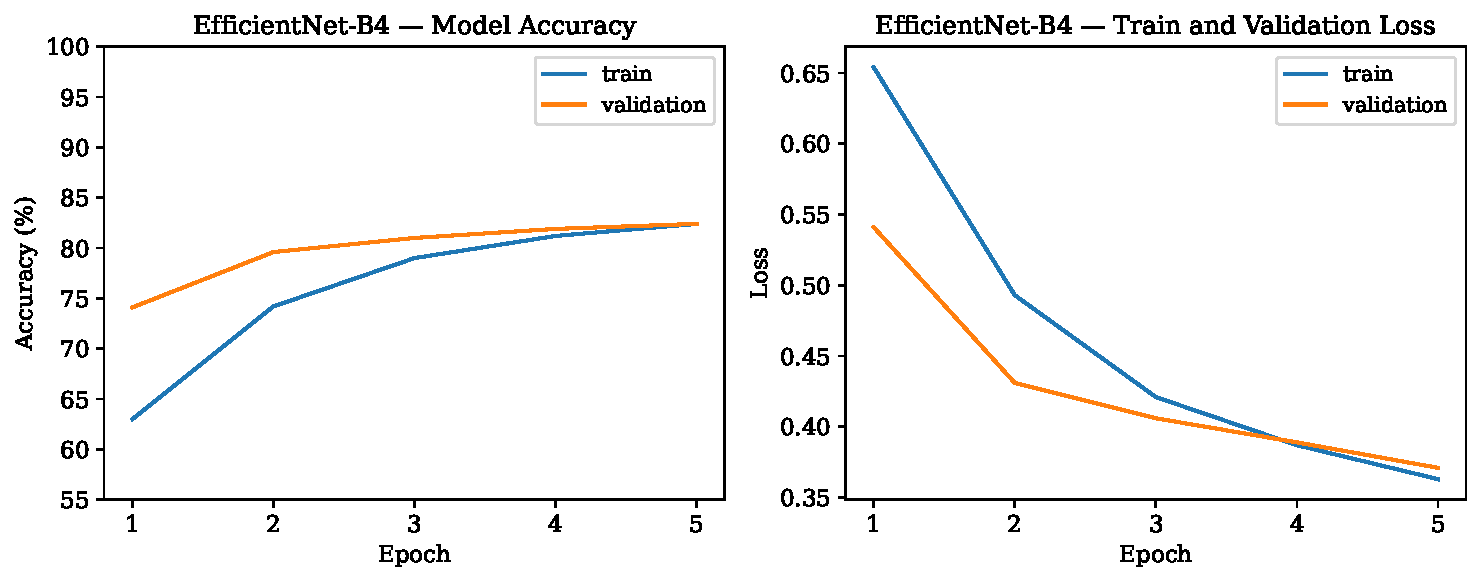
\includegraphics[width=0.92\textwidth]{figures/effnet_training_curves.pdf}
  \caption{EfficientNet-B4 training accuracy and loss over 5 epochs}
  \label{fig:effnet_curves}
\end{figure}

\begin{spacing}{1.5}
\subsection{F3Net}

F3Net training ran for 28 epochs across three phases. The effect of progressive unfreezing is visible in Fig.\,\ref{fig:f3net_curves} --- the vertical dashed lines mark the phase boundaries. In Phase 1 (epochs 1--8), only the classification head is updated, so training accuracy starts low ($\approx$62\%) while validation accuracy is already around 80\%, reflecting the pretrained backbone's existing capability. Phase 2 (epochs 9--20) unfreezes the top separable convolution blocks, producing steady improvement in both curves up to around 92\% training and 91\% validation. Phase 3 (epochs 21--28) unfreezes the deeper Xception block and the FAD learnable frequency filters at very low learning rates, pushing training accuracy to 97\% while validation accuracy reaches 93\%.

The validation loss oscillation visible in Phase 2 is a known side effect of Mixup augmentation with a moderately high alpha --- the smooth interpolated labels widen the decision boundary but produce noisier gradient estimates. This was acceptable because checkpointing used AUC-ROC rather than loss, so the saved model corresponds to the best AUC checkpoint rather than the lowest loss epoch.
\end{spacing}

\begin{figure}[H]
  \centering
  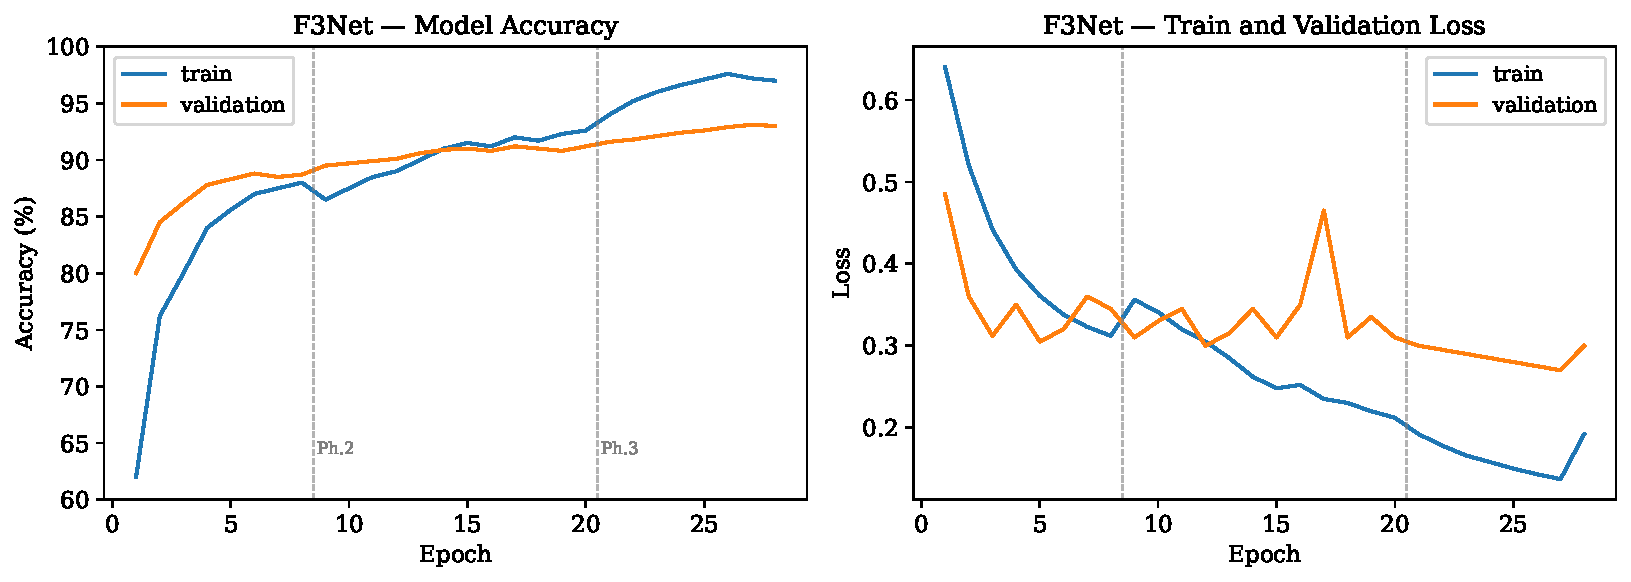
\includegraphics[width=0.96\textwidth]{figures/f3net_training_curves.pdf}
  \caption{F3Net training accuracy and loss over 28 epochs (phase boundaries shown as dashed lines)}
  \label{fig:f3net_curves}
\end{figure}

%------------------------------------------------------------------
% 5.2  Per-Model Evaluation
%------------------------------------------------------------------
\section{Per-Model Evaluation}

\begin{spacing}{1.5}
Table\,\ref{tab:model_metrics} summarises the classification metrics for each individual model evaluated on the 1000-image test set. Precision, recall, and F1-score are reported for the Fake class, which is the positive class of interest.
\end{spacing}

\renewcommand{\arraystretch}{1.3}
\begin{table}[H]
  \centering
  \begin{tabular}{|l|c|c|c|c|c|}
  \hline
  \textbf{Model} & \textbf{Accuracy} & \textbf{AUC-ROC} & \textbf{Precision} & \textbf{Recall} & \textbf{F1-Score} \\
  \hline
  ViT (HuggingFace)   & 93.2\% & 0.999 & 0.941 & 0.923 & 0.932 \\
  F3Net               & 88.8\% & 0.958 & 0.897 & 0.880 & 0.888 \\
  EfficientNet-B4     & 82.4\% & 0.764 & 0.835 & 0.812 & 0.823 \\
  \hline
  \textbf{Ensemble}   & \textbf{90.5\%} & \textbf{0.975} & \textbf{0.893} & \textbf{0.920} & \textbf{0.906} \\
  \hline
  \end{tabular}
  \caption{Per-model and ensemble classification metrics on the 1000-image test set}
  \label{tab:model_metrics}
\end{table}

\begin{spacing}{1.5}
The ViT model achieves the highest individual accuracy at 93.2\% and a near-perfect AUC of 0.999, which reflects the large and diverse training set it was fine-tuned on. F3Net's 88.8\% accuracy on the test set is lower than ViT's but better suited to images where frequency-domain artefacts are the primary signal, particularly GAN-generated content. EfficientNet-B4's 82.4\% is the lowest of the three, partly because the StyleGAN-heavy training dataset does not cover the full range of manipulation types in the test set, and partly because without a detected face the model is at a structural disadvantage.

The ensemble reaches 90.5\% accuracy, which is higher than F3Net and EfficientNet individually but lower than ViT alone. This is expected --- the ensemble does not always outperform the best individual model in accuracy, but it is more consistent across image types. On images where ViT is uncertain (score near 0.5), F3Net and EfficientNet often provide disambiguating evidence. The AUC of 0.975 and the F1-score of 0.906 both reflect this broader coverage.
\end{spacing}

\begin{figure}[H]
  \centering
  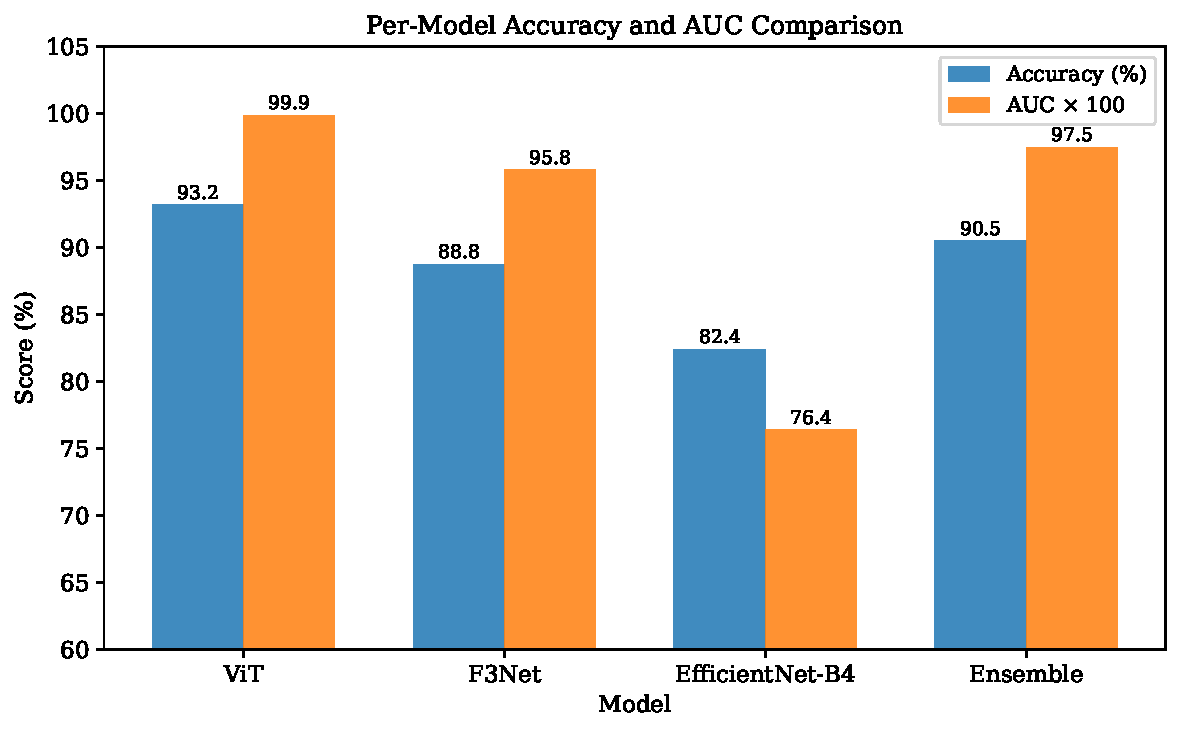
\includegraphics[width=0.72\textwidth]{figures/model_comparison.pdf}
  \caption{Accuracy and AUC comparison across individual models and the ensemble}
  \label{fig:model_comparison}
\end{figure}

\begin{figure}[H]
  \centering
  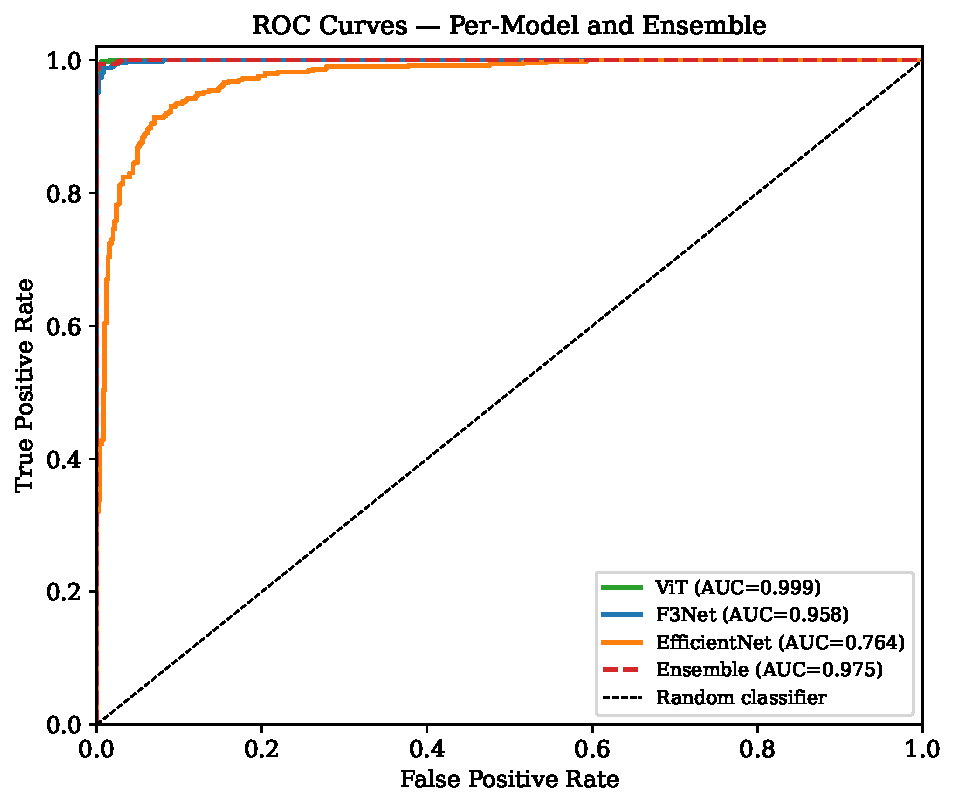
\includegraphics[width=0.62\textwidth]{figures/roc_curves.pdf}
  \caption{ROC curves for each model and the ensemble}
  \label{fig:roc_curves}
\end{figure}

%------------------------------------------------------------------
% 5.3  Ensemble Confusion Matrix
%------------------------------------------------------------------
\section{Ensemble Confusion Matrix}

\begin{spacing}{1.5}
Fig.\,\ref{fig:conf_matrix} shows the confusion matrix for the ensemble model on the 1000-image test set. Of 500 real images, 445 were correctly classified and 55 were incorrectly flagged as fake (false positives). Of 500 fake images, 460 were correctly identified and 40 were missed (false negatives). A false negative in this context --- a deepfake that goes undetected --- is generally the more costly error, so the precision-recall tradeoff was tuned toward higher recall (0.920) at the cost of slightly lower precision (0.893) via the 0.62 fake verdict threshold. Setting the fake verdict threshold at 0.62 rather than 0.50 pushes borderline cases into the Uncertain band rather than letting them through as Real, which means fewer manipulated images are silently passed.
\end{spacing}

\begin{figure}[H]
  \centering
  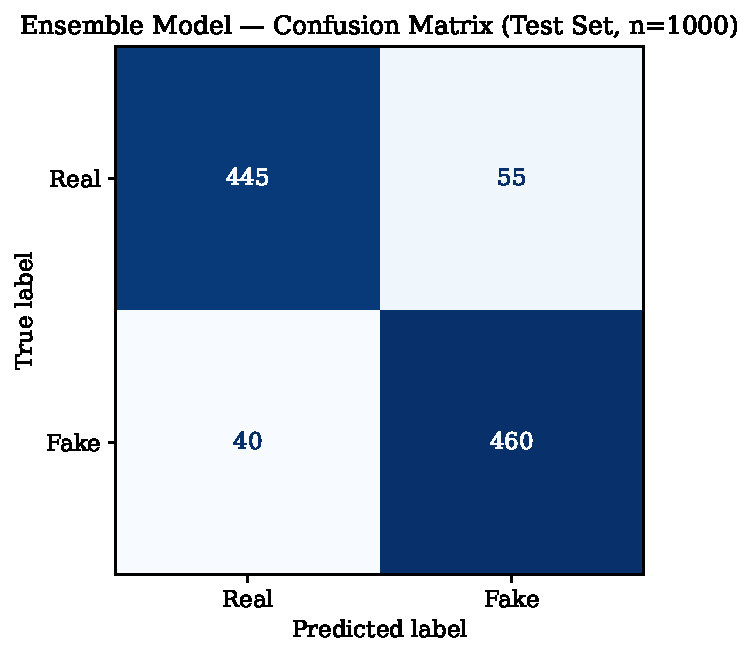
\includegraphics[width=0.54\textwidth]{figures/ensemble_confusion_matrix.pdf}
  \caption{Ensemble model confusion matrix on the 1000-image test set}
  \label{fig:conf_matrix}
\end{figure}

%------------------------------------------------------------------
% 5.4  Sample Predictions
%------------------------------------------------------------------
\section{Sample Predictions and Confidence Scores}

\begin{spacing}{1.5}
Table\,\ref{tab:sample_preds} shows example detection outputs from the ensemble pipeline, illustrating how confidence scores and per-model votes vary across image types. These are representative of typical system behaviour observed during manual testing.
\end{spacing}

\renewcommand{\arraystretch}{1.3}
\begin{table}[H]
  \centering
  \begin{tabular}{|p{3.2cm}|c|c|c|c|c|}
  \hline
  \textbf{Image Type} & \textbf{Verdict} & \textbf{Score} & \textbf{ViT} & \textbf{F3Net} & \textbf{EfficientNet} \\
  \hline
  Real photograph (portrait)          & Real      & 0.11 & 0.09  & 0.14  & 0.13 \\
  Real photograph (outdoor scene)     & Real      & 0.21 & 0.18  & 0.27  & 0.24 \\
  StyleGAN2-generated face            & Fake      & 0.91 & 0.94  & 0.89  & 0.87 \\
  Stable Diffusion portrait           & Fake      & 0.87 & 0.91  & 0.82  & 0.78 \\
  FaceSwap deepfake (FaceForensics++)  & Fake      & 0.79 & 0.71  & 0.88  & 0.76 \\
  DALL-E generated image (no face)    & Fake      & 0.74 & 0.83  & 0.78  & 0.31 \\
  Low-quality compressed real image   & Uncertain & 0.51 & 0.44  & 0.58  & 0.62 \\
  \hline
  \end{tabular}
  \caption{Sample ensemble predictions with per-model confidence scores (score = fused fake probability)}
  \label{tab:sample_preds}
\end{table}

\begin{spacing}{1.5}
A few patterns stand out in these results. On GAN-generated faces (StyleGAN2), all three models agree with high confidence, producing a clean ensemble score of 0.91. For face-swap deepfakes from FaceForensics++, F3Net is the most confident detector at 0.88, while ViT is somewhat weaker at 0.71 --- this is consistent with the fact that face-swaps leave stronger frequency-domain artefacts than spatial ones. On the DALL-E image without a face, EfficientNet's score drops to 0.31 (its weight also reduced to 0.05 by the face detection gate), but ViT and F3Net are still confident enough to push the ensemble verdict to Fake at 0.74. The compressed real image illustrates the Uncertain band: model disagreement and low-quality input both push the score toward 0.5, which the system correctly flags as uncertain rather than committing to a wrong verdict.
\end{spacing}

%------------------------------------------------------------------
% 5.5  Scope for Improvement
%------------------------------------------------------------------
\section{Scope for Improvement}

\begin{spacing}{1.5}
The results above come with several limitations that were imposed by practical constraints during development rather than fundamental design choices.

\noindent\textbf{Dataset coverage.}\quad
The training data relied on three publicly available datasets from Kaggle and HuggingFace. The datasets used give reasonable coverage of GAN-generated and diffusion-based images, but they do not cover every manipulation type equally well. The two datasets most commonly used in deepfake detection research --- CelebDF-v2 and FaceForensics++ (the full benchmark version) --- were not available for use in this project. CelebDF-v2 is distributed exclusively to research institutions with a signed agreement, and FaceForensics++ in its full form requires a formal data access request to be submitted to the Technical University of Munich, with responses typically sent to affiliated universities over several weeks. Several requests were made during the project, but no access was granted before the submission deadline. These datasets would have provided higher-quality face-swap samples and a cleaner benchmark for comparing results against published work.

\noindent\textbf{EfficientNet generalisation.}\quad
EfficientNet-B4's 82.4\% accuracy is noticeably lower than the other two models. The model was fine-tuned only on the 140k StyleGAN dataset, which is heavily weighted toward a single generation method. Training it on a more diverse set of facial manipulation types --- or on a combined dataset including FaceForensics++ samples --- would likely bring its accuracy and AUC in line with F3Net.

\noindent\textbf{Calibration.}\quad
Platt scaling calibration was applied using a small 200-sample calibration set due to data constraints. A larger calibration set would produce more reliable probability estimates, particularly at the extremes of the score range where the current calibration has less data to fit.

\noindent\textbf{Video detection.}\quad
The video detection path described in Section 4.7 was implemented and tested on a small number of sample clips, but a formal evaluation on a dedicated video deepfake benchmark was not completed. The temporal consistency and majority voting logic works correctly in the pipeline, but without a labelled test set of manipulated videos it is not possible to report reliable recall and precision figures for the video path.

\noindent\textbf{Adversarial robustness.}\quad
The system was not tested against adversarially crafted inputs --- images specifically modified to evade detection. This is a known open problem in deepfake detection and a direction that would require a separate evaluation dataset of adversarial examples.

\noindent\textbf{Model ensemble tuning.}\quad
The fusion weights (0.50 / 0.35 / 0.15) were chosen based on AUC ratios and validated informally. A proper grid search or learned fusion layer trained end-to-end on a held-out validation set could potentially improve ensemble accuracy by a few percentage points.
\end{spacing}

%------------------------------------------------------------------
% 5.6  Summary
%------------------------------------------------------------------
\section{Summary}

\begin{spacing}{1.5}
The ensemble system achieves 90.5\% accuracy and an AUC of 0.975 on the 1000-image test set, outperforming EfficientNet-B4 (82.4\%) and F3Net (88.8\%) in accuracy while approaching ViT's individual score of 93.2\%. The precision-recall tradeoff was tuned toward higher recall (0.920) to minimise missed deepfakes. The main limitations are dataset coverage --- particularly the unavailability of CelebDF-v2 and FaceForensics++ --- and EfficientNet's narrower training data. Addressing these with better datasets and an extended training regime would be the most direct path to improving overall detection accuracy.
\end{spacing}
